\chapter{Expert priors in compartments models: bipolar disorder}
\label{applications-prior_level_vals}

Just as priors in the spline model were influential on the estimates
produced for PMS prevalence in
Chapter~\ref{applications-priors_knots_select}, the priors on the
age-specific rates in a compartmental model can be influential on the
estimates.  The situation is more complicated here, however, because
priors on a hazard of one type propagate through to affect the
estimates for all other parameters as well, due to the consistency
enforced by the compartmental model.  In this chapter, we will use the
meta-analysis of bipolar disorder prevalence as an example of the
effects of informative priors on levels of age-specific incidence and
remission hazards.

Bipolar disorder is a mental disorder that causes the experience
of at least one manic (or hypomanic) and one major depressive episode,
interspersed by periods of residual symptoms.  A manic episode is
characterized by elevated, expansive, or irritable mood while a
depressive episode is characterized by depressed mood or loss of
interest in everyday activities.  A shift between episodes is
demarcated by either a change in symptoms to the opposite polarity
or experiences of residual symptoms which are below the threshold
for a manic or depressive episode.  Although residual symptoms can be
less severe than manic and depressive episodes, there is still
considerable disability associated with these periods.  In the case of rapid cycling,
shifts between episodes occur as frequently as four or more shifts
in a given year.  Extreme behavior
changes accompany mood changes, and it is not uncommon for sleeping,
eating or activity patterns to change with manic and depressive
episodes.
While there
is no cure, treatment helps manage mood swings and related
symptoms. \cite{kloos_bipolar_2011, angst_historical_2000, TK_coauthor_ref}

The modeling of bipolar disorder is based on literature describing it
as a chronic illness with little or no complete remission.
The terms `residual' and `remission' have very different implications
for the GBD 2010 study.  A residual state involves less severe
symptoms with lesser disability which still contributes to disease
burden.  Remission is equivalent to a cure rather than a temporary
reduction in symptom levels, thus not contributing to burden.  No studies
were found reporting on complete remission from bipolar disorder as per this definition,
which is consistent with the description in the literature that there
is no cure. \cite{american_psychiatric_association_diagnostic_2000}
In this chapter, analysis
only uses data from the GBD 2010 Study region of North America, High Income,
shown in Figure~\ref{fig:app-bipolar data}.

    \begin{figure}[h]
        \begin{center}
            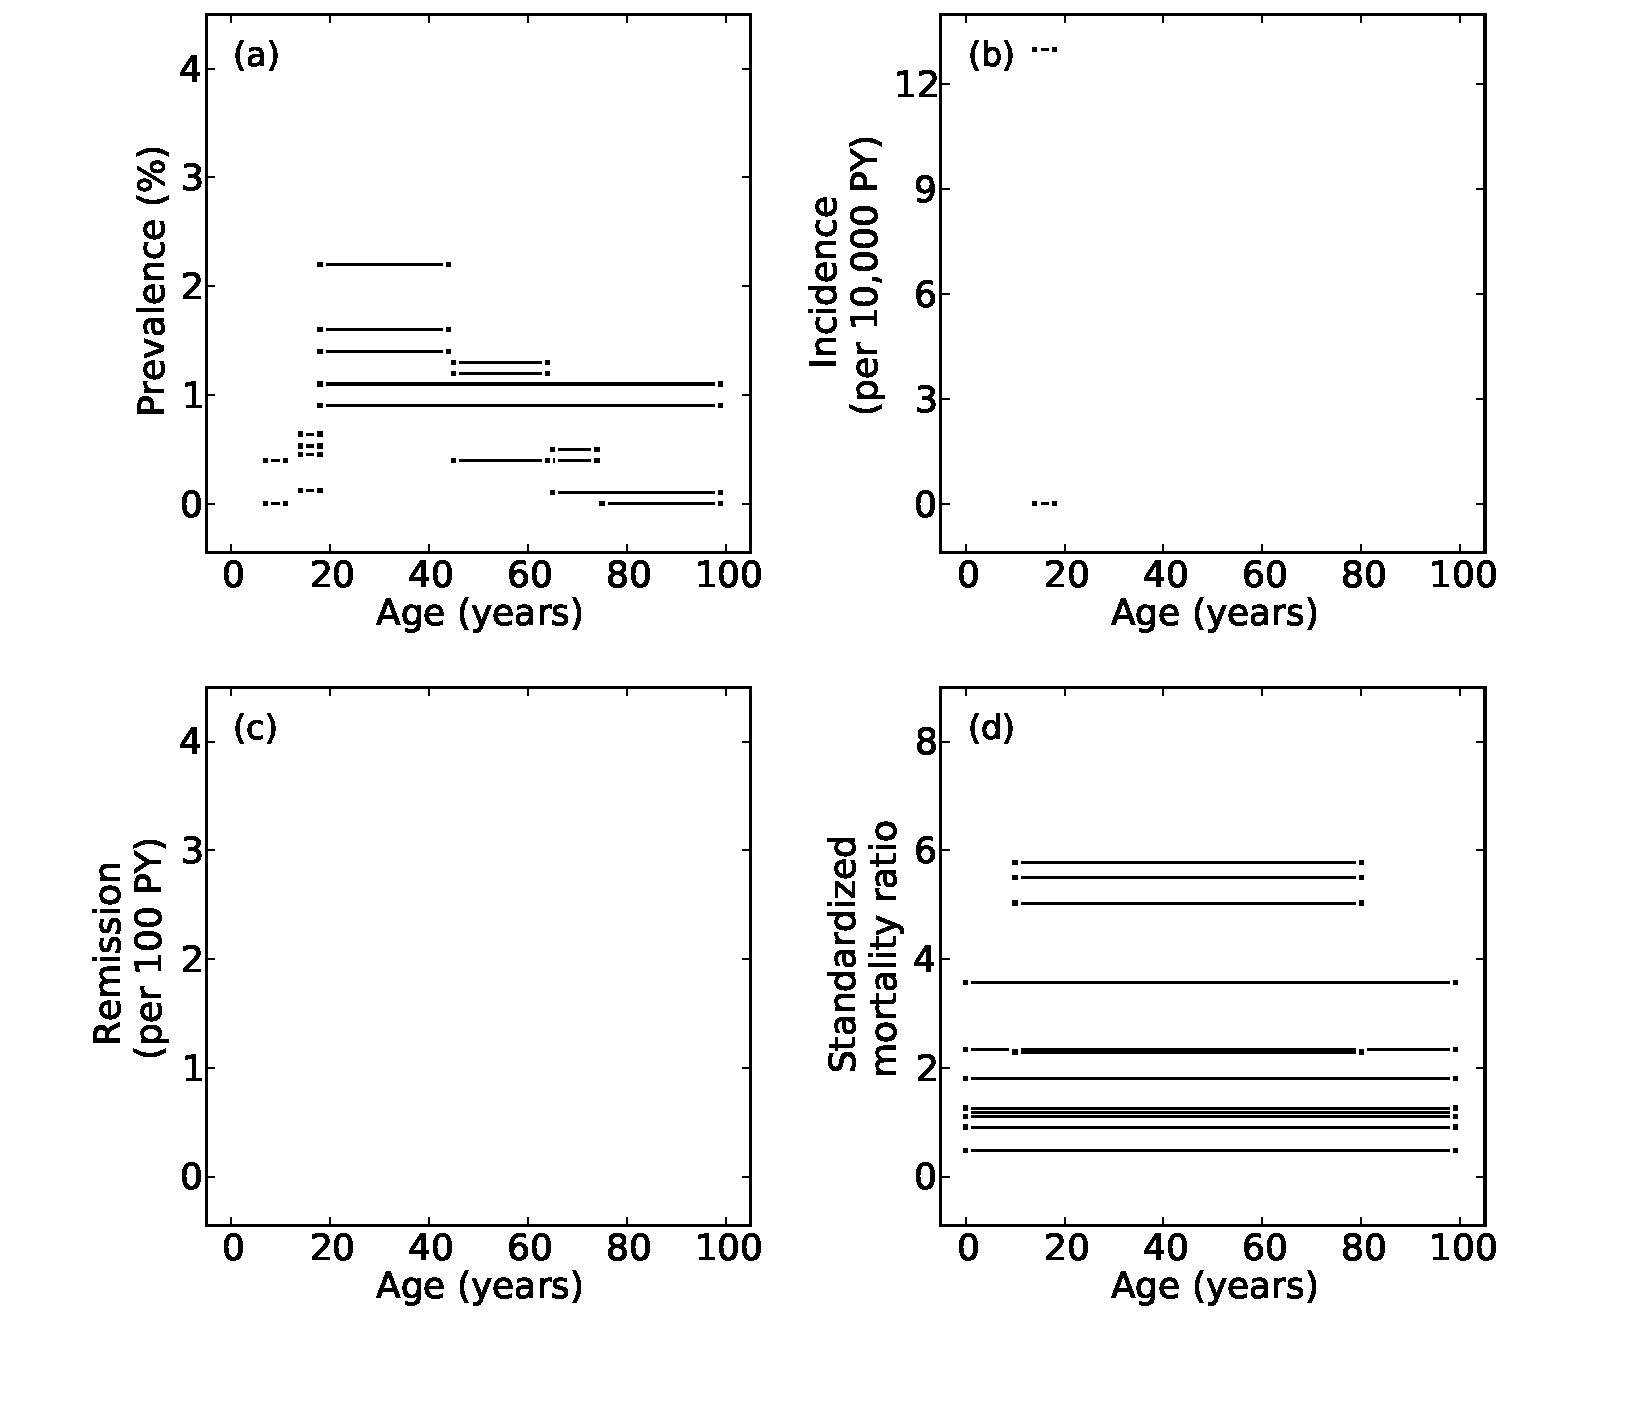
\includegraphics[width=\textwidth]{bipolar-data.pdf}
            \caption{Data collected from systematic review of bipolar
              disorder of (a) prevalence, (b) incidence, (c) remission and
              (d) standardized mortality ration in the GBD 2010 Study
              region of North America, High Income.}
            \label{fig:app-bipolar data}
        \end{center}
    \end{figure}

%\section{Prevalence and Incidence age of onset}
While there is evidence to suggest that bipolar disorder commonly
starts in the mid-teens or early twenties, there is still disagreement
over a minimum age of onset.  Even though symptoms can be tracked back
to childhood, setting a threshold for diagnosis is difficult given
that current diagnostic criteria are based on the adult presentation of
the disorder.  Literature and expert advice suggest that although
pre-pubertal bipolar disorder is rare, there is a possibility it may
exist. \cite{kloos_bipolar_2011, angst_historical_2000}

While expert priors are useful in guiding the modeling process, they
may have unintended effects as discussed in Chapter~\ref{theory-expert_priors}.
Choosing to have no restrictions on the
age of onset, the age-specific prevalence differs greatly, as shown in
Figure~\ref{fig:app-bipolar bounds}.

    \begin{figure}[h]
        \begin{center}
            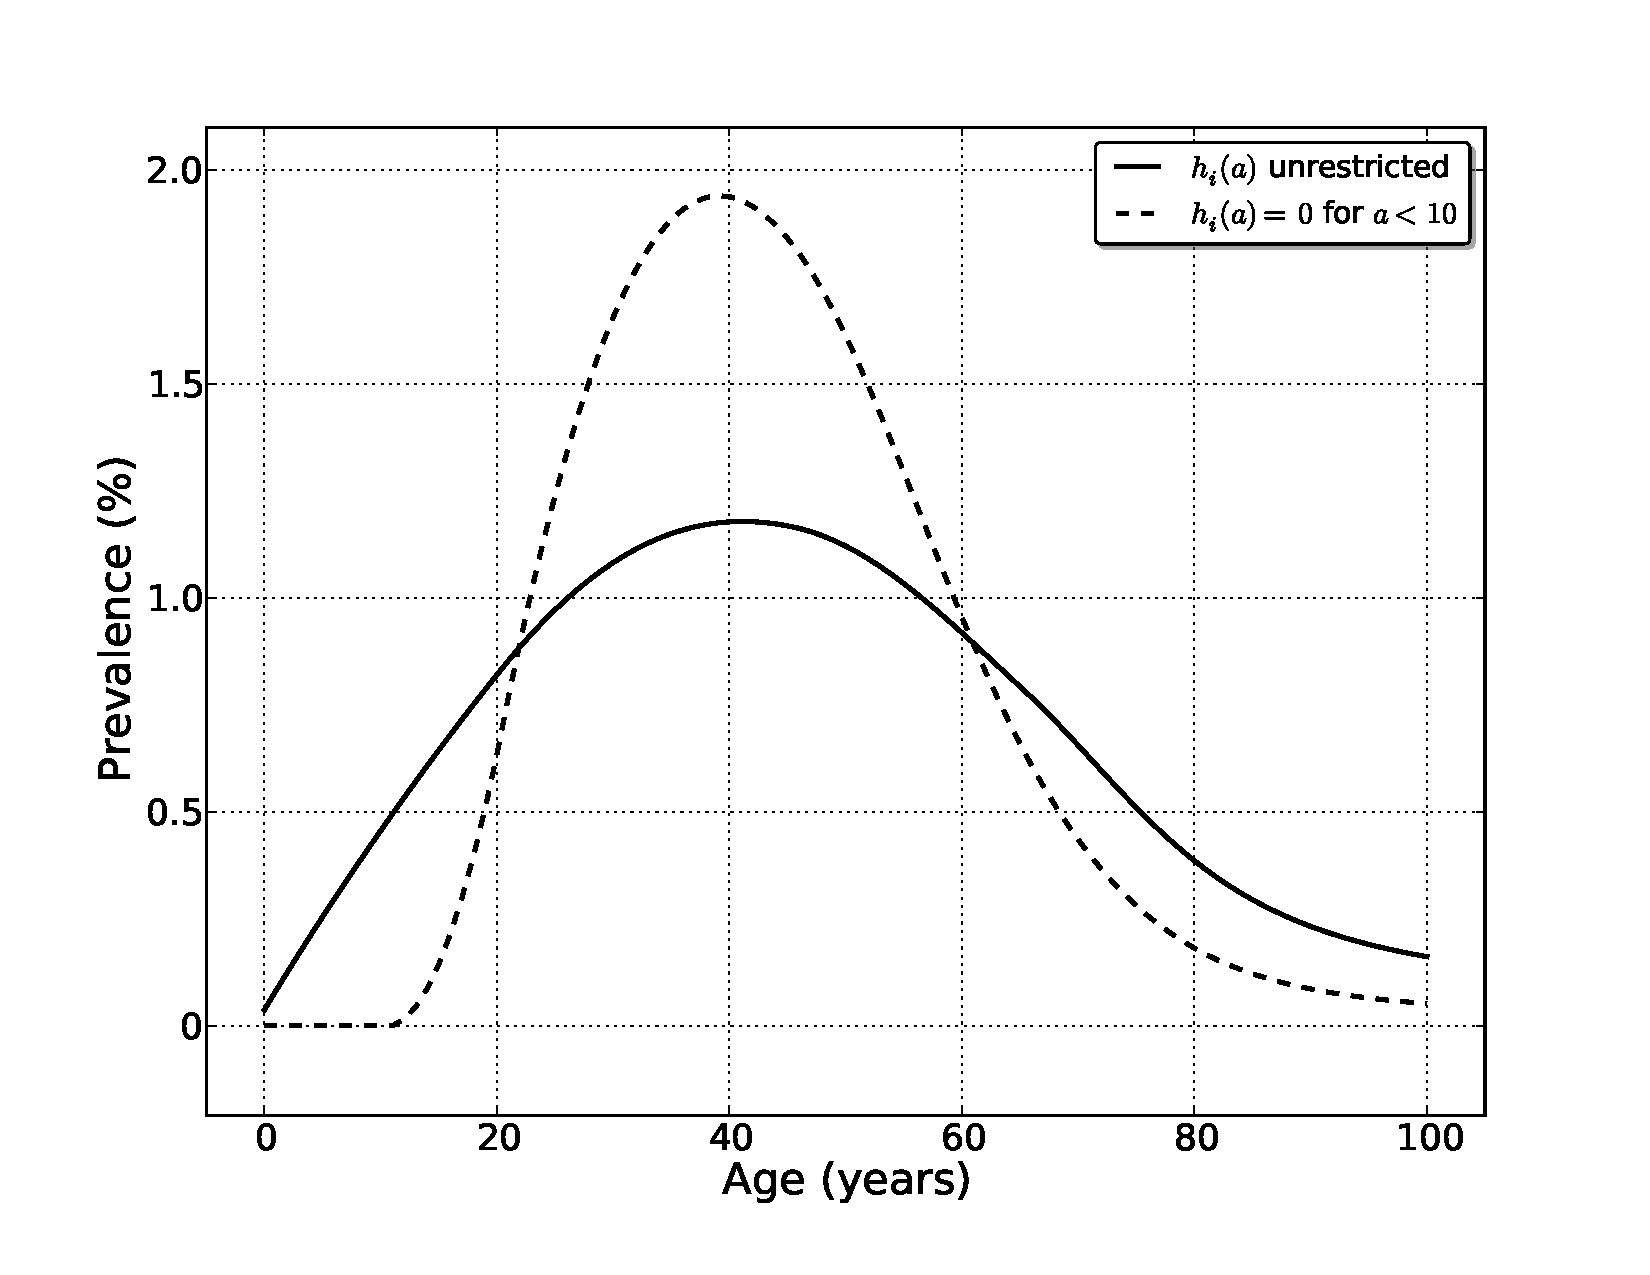
\includegraphics[width=\textwidth]{bipolar-bounds.pdf}
            \caption{Estimates of the prevalence of bipolar disorder
              for males in the GBD 2010 Study region of North America, High Income
              in 1990 using differing priors that limit the age of onset
              in a compartmental model.}
            \label{fig:app-bipolar bounds}
        \end{center}
    \end{figure}

Like the age of onset, little is known about the upper age limit of
bipolar disorder.  Using expert knowledge to set plausible bounds on the
level of disease is useful in modeling noisy data.  However, changes in the upper age
limit may produce unexpected changes as shown in Figure~\ref{fig:app-bipolar onset}.
The prevalence estimates in Figure~\ref{fig:app-bipolar onset} are about
the same because there is enough data to inform the model, but incidence,
remission and excess mortality make subtle changes to account for the prior.

    \begin{figure}[h]
        \begin{center}
            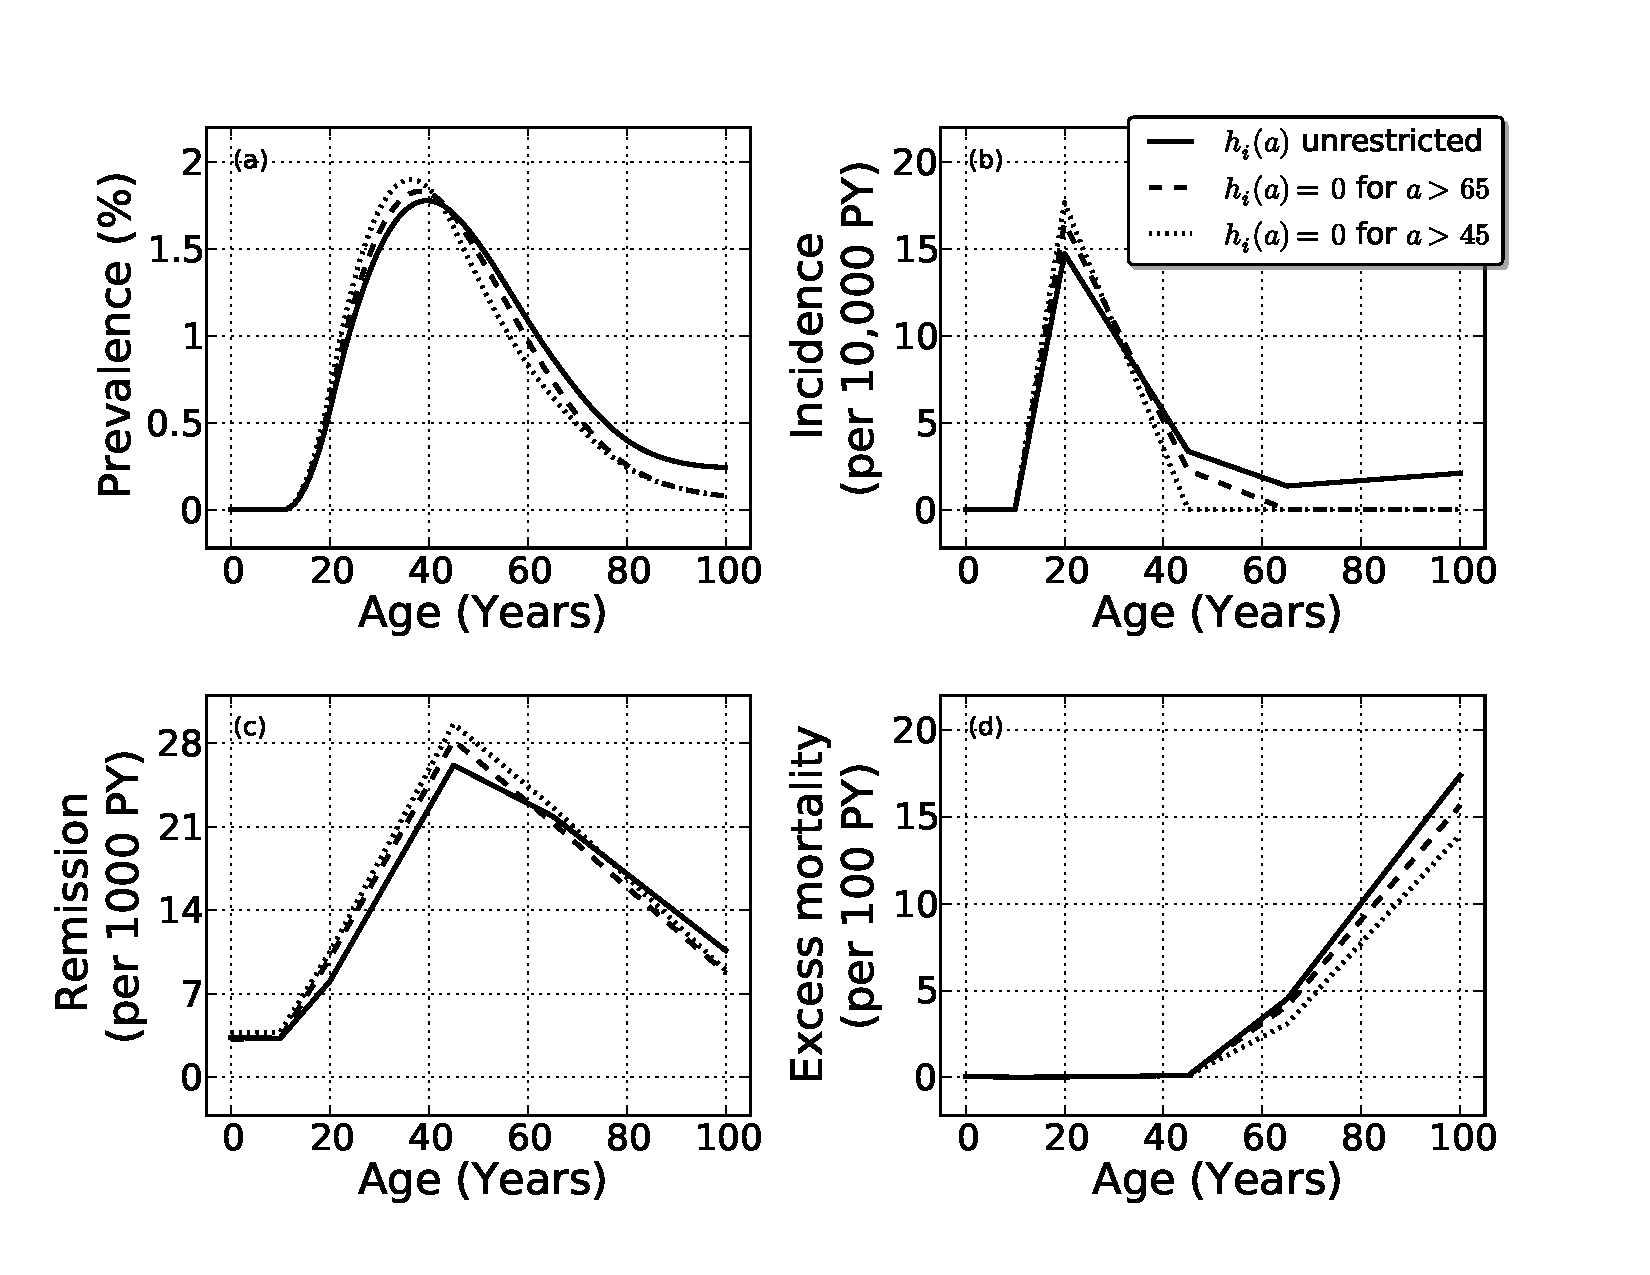
\includegraphics[width=\textwidth]{bipolar-45_65_100.pdf}
            \caption{Estimated (a) prevalence, (b) incidence, (c) remission and
              (d) excess mortality for males with bipolar
              disorder in the GBD 2010 Study region of North America, High Income
              in 1990 using a compartmental model with
              different priors that restrict the upper age limit of
              incidence to 45, 65 or 100.}
            \label{fig:app-bipolar onset}
        \end{center}
    \end{figure}

%\section{Residual v Remission}
In sparse and noisy data, sometimes the changes to account for the prior
are not so subtle, as shown in the sensitivity analysis in
Figure~\ref{fig:app-bipolar remission}.  Here, small changes in the
prior level on remission lead to large changes in the estimated excess mortality.

    \begin{figure}[h]
        \begin{center}
            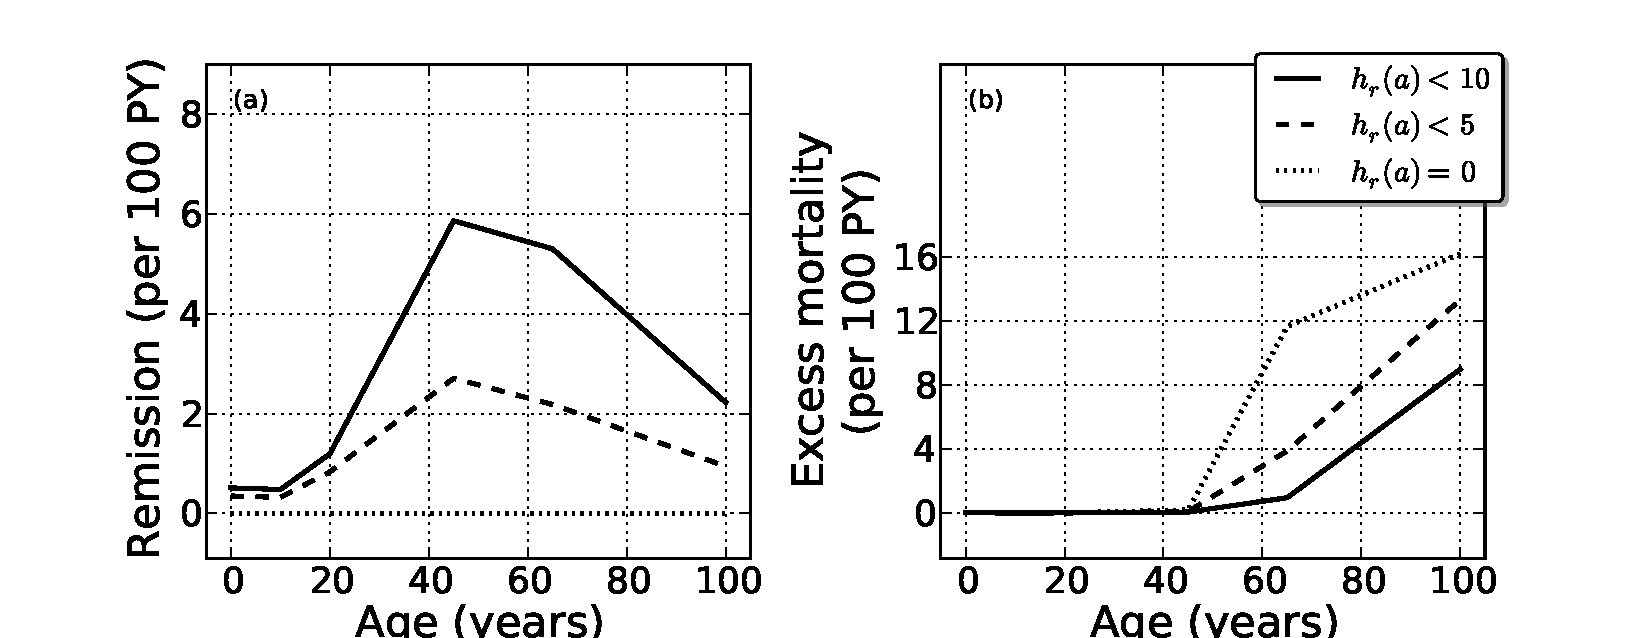
\includegraphics[width=\textwidth]{bipolar-0_5_10.pdf}
            \caption{Estimated (a) remission and (b) excess
              mortality for bipolar disorder in
              males in the GBD 2010 Study region of North America, High Income
              in 1990 in a compartmental model
              with different priors on remission which limit remission
              to 0, 5 or 10 per 100 PY.}
            \label{fig:app-bipolar remission}
        \end{center}
    \end{figure}

The internal consistency in the compartmental model causes modeling
decisions, such as priors on level, for one parameter to propagate and
affect all other parameter estimates.  When working with ample data,
the model estimates are robust to the choice of informative priors on
level.  However, these choices can cause substantial changes to
estimates when working with sparse and noisy data.




